%\documentclass{beamer}
\documentclass[handout]{beamer}
%\documentclass{beamer}
%\usepackage{xeCJK}
\usepackage{ctex}

\usepackage[orientation=landscape,size=custom,width=16,height=12,scale=0.5,debug]{beamerposter}

 % 1. packages

 % ----------- fonts and symbles ---------
\usepackage{amsmath,amssymb,amsfonts,amsthm}
%\usepackage{CJK}
\usepackage{dsfont}
\usepackage{mathrsfs}
\usepackage{eucal} % for \mathcal

%\renewcommand{\rmdefault}{ptm}


%\usepackage{fontspec}
%\newfontfamily\monaco{Monaco}

%\usepackage{mathbbold} %,bbold

 \usepackage{textcomp} % for \textnormal{\textperthousand}
% -----------------





%\usepackage{slashbox}
%\usepackage[margin=2.2cm]{geometry} % |geometry| package clash with |booktabs| package
%\usepackage{cases}
% -------- tables -------
\usepackage{booktabs} % for \toprule, \bottomrule
\usepackage{tabularx}
\usepackage{multirow}
% --------- figures ---------
\usepackage{graphicx}
% ---------- algorithms -------
\usepackage{algorithm}
\usepackage{algorithmic}
%\usepackage{footnote}
    % |footnote| package occurs error:
    % Runaway argument?
    % \def \insertfootnotetext {\@@ }\def \insertfootnotemark {\@makefnmark \ETC.

\usepackage{listings}

\usepackage[linewidth=1pt]{mdframed} % for  mdframe environment




 \usepackage{color}
 \usepackage{xcolor}     %¸ßÁÁʹÓõÄÑÕÉ«

\usepackage{setspace}
%%\usepackage{type1cm}
\usepackage{adjustbox} % for \adjustbox

\usepackage{accsupp}
\newcommand{\emptyaccsupp}[1]{\BeginAccSupp{ActualText={}}#1\EndAccSupp{}}




%%   figures and tables
\graphicspath{{figure/}}


% 2. new commands

% 2.0 common commands
%\newcommand{\bc}{\begin{center}}
%\newcommand{\ec}{\end{center}}
%\newcommand{\ba}{\begin{array}}
%\newcommand{\ea}{\end{array}}
%\newcommand{\be}{\begin{equation}}
%\newcommand{\ee}{\end{equation}}

% 2.1 colors
\definecolor{dgrey}{rgb}{0.30,0.30,0.30}
\definecolor{lred}{rgb}{0.50,0.00,0.50}
\definecolor{lblue}{rgb}{0.8,0.8,1}
\definecolor{dred}{rgb}{0.6,0,0}
\definecolor{dblue}{rgb}{0,0,0.5}
\definecolor{dgrey}{rgb}{0.35,0.35,0.35}
\definecolor{rred}{rgb}{0.9,0,0}
\definecolor{mylblue}{rgb}{0.3,0.2, 0.8}

\definecolor{commentcolor}{RGB}{85,139,78}
\definecolor{stringcolor}{RGB}{206,145,108}
\definecolor{keywordcolor}{RGB}{34,34,250}
\definecolor{backcolor}{RGB}{220,220,220}

\newcommand{\blue}[1]{{\color{blue}#1}}
\newcommand{\dblue}[1]{{\color{dblue}#1} }
\newcommand{\red}[1]{{\color{red}#1}}
\newcommand{\dred}[1]{{\color{dred}#1}}
\newcommand{\cyan}[1]{{\color{cyan}#1}}
\newcommand{\bfblue}[1]{\textbf{\color{dblue}#1} }
\newcommand{\bfred}[1]{\textbf{\color{dred}#1} }
\newcommand{\green}[1]{{\color{green}#1}}
%\newcommand{\alert}[1]{{\color{red}#1}}
\newcommand{\black}[1]{{\color{black}#1}}
\newcommand{\light}[1]{{\color{blue}\textbf{#1}}}
\newcommand{\hot}[1]{{\color{dred}#1}}
 \newcommand{\highlight}[1]{ \textbf{\color{mylblue}#1}}
 \newcommand{\important}[1]{{\color{red}#1}} % for highlighting  some words

 \newcommand{\mystar}{\dred{$^{\clubsuit}$ }}
  \newcommand{\doublestar}{\dred{$^{\clubsuit\clubsuit}$ }}

\newcommand{\mynote}[1]{{\footnotesize \color{mylblue}#1}}

 \newcommand{\hint}[1]{{\small \color{mylblue}#1}}
\newcommand{\smallhint}[1]{{\small \color{dgrey}#1}}
\newcommand{\footnotehint}[1]{{\footnotesize \color{dgrey}#1}}
\newcommand{\tinyhint}[1]{{\tiny \color{dgrey}#1}}
\newcommand{\mytitle}[1]{\medskip{\large \textbf{\color{mylblue}#1}}}
\newcommand{\normaltitle}[1]{\medskip{ \textbf{\color{mylblue}#1}}}

%\newcommand{\head}[1]{\textbf{\large\color{blue}#1}}
%\newcommand{\heading}[1]{\textbf{\large\color{blue}#1}}

\newcommand{\myfbox}[2]{ \bigskip \begin{center} \fbox{\parbox{#1}{ #2  }} \end{center}\bigskip }

\newcommand{\myvar}[1]{}
%\newcommand{\mynote}[1]{#1}

% 2.2 mathematical symbols

\newcommand{\drightarrow}{\stackrel{d.}{\rightarrow}}
\newcommand{\prightarrow}{\stackrel{p.}{\rightarrow}}
\newcommand{\bernoulli}{\textnormal{Ber}}
\newcommand{\cov}{\mathsf{Cov}}
\newcommand{\corr}{\mathbf{Corr}}
\newcommand{\regret}{\textnormal{Regret}}
\newcommand{\conv}{\textnormal{conv}}
\newcommand{\dotdiv}{\stackrel{\centerdot}{-}}
\newcommand{\dom}{\textnormal{dom}}
\newcommand{\convergenceinprob}{\stackrel{P}{\rightarrow}}
\newcommand{\convergenceindist}{\rightsquigarrow}
\newcommand{\probability}{\mathbb{P}}
\newcommand{\expectation}{\mathbb{E}}
\newcommand{\epi}{\textnormal{epi}}
\newcommand{\variance}{\mathbb{V}}
\newcommand{\var}[1]{\mathbb{V}(#1)}
\newcommand{\covariance}{\mathsf{Cov}}
\newcommand{\empiricalrisk}[1]{\hat{R}(#1)}
\newcommand{\expectedrisk}[1]{R(#1)}
\newcommand{\mgf}[1]{\psi_{#1}(\lambda)}
\newcommand{\mgfexpansion}[1]{\expectation[e^{\lambda#1}]}
\newcommand{\mgfmultivariate}[1]{\expectation[e^{\lambda^\transpose#1}]}
\newcommand{\transpose}{{\mathsf{T}}}
\newcommand{\real}{\mathbb{R}}
\newcommand{\gaussian}[2]{\mathcal{N}(#1,#2)}
\newcommand{\subGaussian}[1]{\mathsf{subG}(#1)}
\newcommand{\indicator}[1]{\mathbb{I}[#1]}
\newcommand{\x}[1]{x^{(#1)}}
\newcommand{\y}[1]{y^{(#1)}}
\newcommand{\z}[1]{z^{(#1)}}
\newcommand{\feature}{x}
\newcommand{\response}{y}
\newcommand{\supofempiricalprocess}{\|\mathbb{P}_n-\mathbb{P}\|_{\decisionspace}}
\newcommand{\decisionspace}{\mathscr{F}}
\newcommand{\decisionfunction}{f}
\newcommand{\featurespace}{\mathcal{X}}
\newcommand{\classifierestimate}{\widehat{h}}
\newcommand{\classifiertrue}{h^\star}
\newcommand{\classifier}{h}
\newcommand{\hypothesisclass}{\mathcal{H}}
\newcommand{\dataset}{\mathcal{D}}
\newcommand{\defineas}{\stackrel{\textnormal{def}}{=}}
\newcommand{\rademachercomplexity}[1]{\mathsf{Rad}_n\left(#1\right)}
\newcommand{\loss}{\ell}
\newcommand{\composite}{\circ}
\newcommand{\convexhull}{\mathsf{conv}}
\newcommand{\norm}[2][2]{\|#2\|_{#1}}
\newcommand{\shatteringcoefficient}[2]{\mathcal{S}(#1,#2)}
\newcommand{\vcdimension}[1]{\mathsf{VC}\left(#1\right)}
\newcommand{\rank}{\mathsf{rank}}
\newcommand{\innerproduct}[2]{\left\langle #1, #2\right\rangle}
\newcommand{\modelparameter}{\theta}
\newcommand{\ball}[3][]{\mathcal{B}_{{#1}}\left(#2,#3\right)}
\newcommand{\metric}{d}
\newcommand{\coveringnumber}[4][]{N_{{#1}}\left(#2,#3,#4\right)}
\newcommand{\trace}{\textnormal{tr}}
\newcommand{\std}{\textnormal{std}}
\newcommand{\sgn}{\textnormal{sign}}
%\renewcommand{\span}{\textnormal{span}}

 % do not overwrite the existing command \span
 % as it leads to an error of
 %  "Missing # Inserted in Alignment Preamble" for ``align'' environment

\newcommand{\myspan}{\textnormal{span}}

%%%
\newcommand{\rightarrowd}{\stackrel{d}{\rightarrow}}
\newcommand{\rightarrowp}{\stackrel{p}{\rightarrow}}
\newcommand{\defeq}{ \stackrel{\textnormal{def}}{=}}
\newcommand{\proj}{ \textnormal{Proj}}
\newcommand{\dist}{\textnormal{dist}}

\newcommand{\argmax}{\textnormal{argmax}}
\newcommand{\argmin}{\textnormal{argmin}}
\newcommand{\subg}{\textnormal{subG}}


 \newcommand{\bba}{\mathbb{A}}
\newcommand{\bbb}{\mathbb{B}}
\newcommand{\bbc}{\mathbb{C}}
\newcommand{\bbd}{\mathbb{D}}
\newcommand{\bbe}{\mathbb{E}}
\newcommand{\bbf}{\mathbb{F}}
\newcommand{\bbg}{\mathbb{G}}
\newcommand{\bbh}{\mathbb{H}}
\newcommand{\bbi}{\mathbb{I}}
\newcommand{\bbj}{\mathbb{J}}
\newcommand{\bbk}{\mathbb{K}}
\newcommand{\bbl}{\mathbb{L}}
\newcommand{\bbm}{\mathbb{M}}
\newcommand{\bbn}{\mathbb{N}}
\newcommand{\bbo}{\mathbb{O}}
\newcommand{\bbp}{\mathbb{P}}
\newcommand{\bbq}{\mathbb{Q}}
\newcommand{\bbr}{\mathbb{R}}
\newcommand{\bbs}{\mathbb{S}}
\newcommand{\bbt}{\mathbb{T}}
\newcommand{\bbu}{\mathbb{U}}
\newcommand{\bbv}{\mathbb{V}}
\newcommand{\bbw}{\mathbb{W}}
\newcommand{\bbx}{\mathbb{X}}
\newcommand{\bby}{\mathbb{Y}}
\newcommand{\bbz}{\mathbb{Z}}

\newcommand{\bfa}{\mathbf{a}}
\newcommand{\bfb}{\mathbf{b}}
\newcommand{\bfc}{\mathbf{c}}
\newcommand{\bfd}{\mathbf{d}}
\newcommand{\bfe}{\mathbf{e}}
\newcommand{\bff}{\mathbf{f}}
\newcommand{\bfg}{\mathbf{g}}
\newcommand{\bfh}{\mathbf{h}}
\newcommand{\bfi}{\mathbf{i}}
\newcommand{\bfj}{\mathbf{j}}
\newcommand{\bfk}{\mathbf{k}}
\newcommand{\bfl}{\mathbf{l}}
\newcommand{\bfm}{\mathbf{m}}
\newcommand{\bfn}{\mathbf{n}}
\newcommand{\bfo}{\mathbf{o}}
\newcommand{\bfp}{\mathbf{p}}
\newcommand{\bfq}{\mathbf{q}}
\newcommand{\bfr}{\mathbf{r}}
\newcommand{\bfs}{\mathbf{s}}
\newcommand{\bft}{\mathbf{t}}
\newcommand{\bfu}{\mathbf{u}}
\newcommand{\bfv}{\mathbf{v}}
\newcommand{\bfw}{\mathbf{w}}
\newcommand{\bfx}{\mathbf{x}}
\newcommand{\bfy}{\mathbf{y}}
\newcommand{\bfz}{\mathbf{z}}

\newcommand{\bfA}{\mathbf{A}}
\newcommand{\bfB}{\mathbf{B}}
\newcommand{\bfC}{\mathbf{C}}
\newcommand{\bfD}{\mathbf{D}}
\newcommand{\bfE}{\mathbf{E}}
\newcommand{\bfF}{\mathbf{F}}
\newcommand{\bfG}{\mathbf{G}}
\newcommand{\bfH}{\mathbf{H}}
\newcommand{\bfI}{\mathbf{I}}
\newcommand{\bfJ}{\mathbf{J}}
\newcommand{\bfK}{\mathbf{K}}
\newcommand{\bfL}{\mathbf{L}}
\newcommand{\bfM}{\mathbf{M}}
\newcommand{\bfN}{\mathbf{N}}
\newcommand{\bfO}{\mathbf{O}}
\newcommand{\bfP}{\mathbf{P}}
\newcommand{\bfQ}{\mathbf{Q}}
\newcommand{\bfR}{\mathbf{R}}
\newcommand{\bfS}{\mathbf{S}}
\newcommand{\bfT}{\mathbf{T}}
\newcommand{\bfU}{\mathbf{U}}
\newcommand{\bfV}{\mathbf{V}}
\newcommand{\bfW}{\mathbf{W}}
\newcommand{\bfX}{\mathbf{X}}
\newcommand{\bfY}{\mathbf{Y}}
\newcommand{\bfZ}{\mathbf{Z}}


\newcommand{\bfSigma}{\mathbf{\Sigma}}
\newcommand{\bfrho}{\mathbf{\rho}}

\newcommand{\cala}{\mathcal{A}}
\newcommand{\calb}{\mathcal{B}}
\newcommand{\calc}{\mathcal{C}}
\newcommand{\cald}{\mathcal{D}}
\newcommand{\cale}{\mathcal{E}}
\newcommand{\calf}{\mathcal{F}}
\newcommand{\calg}{\mathcal{G}}
\newcommand{\calh}{\mathcal{H}}
\newcommand{\cali}{\mathcal{I}}
\newcommand{\calj}{\mathcal{J}}
\newcommand{\calk}{\mathcal{K}}
\newcommand{\call}{\mathcal{L}}
\newcommand{\calm}{\mathcal{M}}
\newcommand{\caln}{\mathcal{N}}
\newcommand{\calo}{\mathcal{O}}
\newcommand{\calp}{\mathcal{P}}
\newcommand{\calq}{\mathcal{Q}}
\newcommand{\calr}{\mathcal{R}}
\newcommand{\cals}{\mathcal{S}}
\newcommand{\calt}{\mathcal{T}}
\newcommand{\calu}{\mathcal{U}}
\newcommand{\calv}{\mathcal{V}}
\newcommand{\calw}{\mathcal{W}}
\newcommand{\calx}{\mathcal{X}}
\newcommand{\caly}{\mathcal{Y}}
\newcommand{\calz}{\mathcal{Z}}


% 3. theorem and environments

%\newtheorem{theorem}{Theorem}%[section]
\newtheorem{proposition}{Proposition}%[section]
%\newtheorem{property}{Property}%[section]
%\newtheorem{lemma}{Lemma}%[section]
%\newtheorem{corollary}{Corollary}%[section]
%\newtheorem{definition}{Definition}%[section]
%\newtheorem{example}{Example}%[section]
%\newtheorem{remark}{Remark}%[section]
%\newtheorem{note}{Note}%[section]
%\newtheorem{problem}{Problem}%[section]
\newtheorem{exercise}{Exercise}
%\newtheorem{assumption}{Assumption}
\newtheorem*{lemma_star}{Lemma}
\newtheorem*{theorem_star}{Theorem}

%\newenvironment{summary}[1][Summary]{\par\medskip   \color{dred}\textbf{\large#1. } }{ \medskip}
%\newenvironment{remark}[1][Remark]{\par\medskip  \begin{small} \color{dblue}\textbf{#1. } }{ \end{small}\medskip}
%\renewenvironment{proof}[1][Proof]{\noindent\textbf{#1.} }{\mbox{} \hfill{\small\textrm{$\Box$}}\vspace{1ex}}
% \newenvironment{answer}[1][Answer]{\par\medskip \color{dblue}\textbf{\large#1. }}{ \medskip}

\newenvironment{summary}[1][总结]{\par\medskip   \color{dred}\textbf{\large#1 } }{ \medskip}
\newenvironment{remark}[1][注意]{\par\medskip   \color{dblue}\textbf{\large#1 } }{ \medskip}
\newenvironment{footnoteremark}{ \color{dblue}\begin{footnotesize} }{\end{footnotesize}}
\renewenvironment{proof}[1][证明]{\noindent\textbf{#1.} }{\mbox{} \hfill{\small\textrm{$\Box$}}\vspace{1ex}}
 \newenvironment{question}[1][Q.]{\par\medskip {\color{lred}\large#1}}{ \medskip}
 \newenvironment{answer}[1][Answer]{\par\medskip \color{dblue}\textbf{\large#1 }}{ \medskip}

% 4. beamer setting




%\newtheorem{definition}{\textbf{¶¨Òå}}[section]
%\newtheorem{proposition}[definition] { \textbf{ÃüÌâ}}
%\newtheorem{lemma}[definition] { \textbf{ÒýÀí}}
%\newtheorem{theorem}[definition]{ \textbf{¶¨Àí}}
%\newtheorem{corollary}[definition] { \textbf{ÍÆÂÛ}}
%\newtheorem{remark}[definition] { \textbf{×¢}}
%\newtheorem{example}[definition] { \textbf{Àý}}

%\newcommand{\shadow}[1]{\begin{center}
%\bf{\textcolor{dblue}{\shadowbox{\parbox{3.8in}
% {\textcolor{red}
% {\vspace{1mm}#1}}}}}
%\end{center}}
%
%\newcommand{\head}[1]{\begin{center}
%\bf{\textcolor{dblue}{\shadowbox{\parbox{3.8in}
% {\textcolor{dred}
% {\vspace{1mm}#1}}}}}
%\end{center}}
%
%
%\newcommand{\heading}[1]{%
%  \begin{center}
%    \large\bf
%    \shadowbox{#1}%
%  \end{center}
%\vspace{1ex minus 1ex}}

% set  space above and below math equations in display style

\expandafter\def\expandafter\normalsize\expandafter{%
    \normalsize
    \setlength\abovedisplayskip{1.5ex}
    \setlength\belowdisplayskip{1.2ex}
    \setlength\abovedisplayshortskip{0.5ex}
    \setlength\belowdisplayshortskip{0.5ex}
}

% Ìí¼ÓÒ³Âë´úÂ룬¹È¸èÕÒµ½µÄ¡£
\addtobeamertemplate{navigation symbols}{}{%
    %\usebeamerfont{footline}%
    %\usebeamercolor[fg]{footline}%
    \setbeamercolor{footline}{fg=blue}
    \setbeamerfont{footline}{series=\bfseries}
    \hspace{1em}%
    \normalsize{\insertframenumber/\inserttotalframenumber}
}

% section numbering
\setbeamertemplate{section in toc}[sections numbered]
\setbeamertemplate{subsection in toc}[subsections numbered]



\lstset{                        %¸ßÁÁ´úÂëÉèÖÃ
%basicstyle=\small, % print whole listing small
%basicstyle=\footnotesize\sffamily, % print whole listing small
basicstyle=\footnotesize\rmfamily, % print whole listing small
%basicstyle=\rmfamily, % print whole listing small
    language=python,                    %PythonÓï·¨¸ßÁÁ
    %linewidth=0.9\linewidth,            %Áбílist¿í¶È
    %basicstyle=\ttfamily,              %ttÎÞ·¨ÏÔʾ¿Õ¸ñ
    commentstyle=\color{commentcolor},  %×¢ÊÍÑÕÉ«
    keywordstyle=\color{keywordcolor},  %¹Ø¼ü´ÊÑÕÉ«
    stringstyle=\color{stringcolor},    %×Ö·û´®ÑÕÉ«
    %showspaces=true,                   %ÏÔʾ¿Õ¸ñ
    numbers=left,                       %ÐÐÊýÏÔʾÔÚ×ó²à
    %numberstyle=\tiny\emptyaccsupp,     %ÐÐÊýÊý×Ö¸ñʽ
    numberstyle=\tiny,                  %ÐÐÊýÊý×Ö¸ñʽ
    numbersep=5pt,                      %Êý×Ö¼ä¸ô
    frame=single,                       %¼Ó¿ò
    framerule=0pt,                      %²»»®Ïß
    %escapeinside=@@,                    %ÌÓÒݱêÖ¾
    escapeinside=``,                    %ÌÓÒݱêÖ¾
    emptylines=1,                       %
    xleftmargin=3em,                    %list×ó±ß¾à
    backgroundcolor=\color{backcolor},  %ÁÐ±í±³¾°É«
    tabsize=4,                          %ÖƱí·û³¤¶ÈΪ4¸ö×Ö·û
    %gobble=4                            %ºöÂÔÿÐдúÂëÇ°4¸ö×Ö·û
    breaklines=true,
    extendedchars=false
    }

\lstdefinestyle{numbers}{numbers=left, stepnumber=1, numberstyle=\tiny, numbersep=10pt}
 \lstdefinestyle{nonumbers}{numbers=none}

\newcommand{\alertcode}[1]{{\color{red}#1}} % used for alerting codes

%\lstset{numbers=left, numberstyle=\tiny,
%keywordstyle=\color{blue!70},
%commentstyle=\color{red!50!green!50!blue!50},
%frame=shadowbox,
%rulesepcolor=\color{red!20!green!20!blue!20},
%escapeinside=``,
%framesep = 2ex,
%rulesep = 1ex
%%framexrightmargin= 1em %
%}


% Vary the color applet  (try out your own if you like)
\colorlet{structure}{red!65!black}

%\beamertemplateshadingbackground{yellow!50}{white}


%\setbeamerfont{normal text}{family=\rmfamily}
%\setbeamerfont{frametitle}{family=\rmfamily}

% Changing the fonts: this will make the slides more readable and the math look like regular tex math
\usefonttheme{serif}



% set spaces

\setstretch{1.2}  % ÉèÖÃÐоà

\addtobeamertemplate{block begin}{\setlength\abovedisplayskip{0pt}} % reduce the large space before a block

% set section number styles



\newcommand{\secno}{Sec.\,\thesection\ }
\newcommand{\subsecno}{Sec.\,\thesubsection\ }

% set logo

 \pgfdeclareimage[width=1.0]{small-logo}{SMaLL.jpg}
%
 \logo{\vbox{\vskip0.1 \hbox{\pgfuseimage{small-logo}}}}

% set math equation fontsize

 \makeatletter
\DeclareMathSizes{\f@size}{10}{5}{5}
\makeatother

% for chinese section name
\hypersetup{CJKbookmarks=true}


%\graphicspath{{./figure/}}

%\usepackage{hyperref}
%\hypersetup{hidelinks,
%	colorlinks=true,
%	allcolors=black,
%	pdfstartview=Fit,
%	breaklinks=true}
	
\begin{document}
\hypersetup{CJKbookmarks=true}
%\begin{CJK*}{GBK}{kai}

\lstdefinestyle{numbers}{numbers=left, stepnumber=1, numberstyle=\tiny, numbersep=10pt}
\lstdefinestyle{nonumbers}{numbers=none}
	
\addtobeamertemplate{block begin}{\setlength\abovedisplayskip{0pt}}

\setbeamertemplate{itemize items}{\color{black}$\bullet$}
	
%\title[Numerical Optimization]{Part1-2 凸优化--Convex Sets}

\title[最优化模型与算法]{第1章\,凸集合}
	
\bigskip
	
\author[]{
		 \underline{SMaLL} 
	}
	
\institute[CUP]{
		\inst{1}
		中国石油大学(华东)\\
		SMaLL 课题组   \\
		\blue{small.sem.upc.edu.cn}\\
		liangxijunsd@163.com \\ 
	 
}
		
\date[2023]{\small    2023}
		
\subject{convex optimization}
	
\frame{\titlepage}
	
%\frame{
%	\frametitle{}
%	\tableofcontents[hideallsubsections]
%}
\section{第1章\,凸集合}

\setcounter{section}{1}

\AtBeginSection[]{
\begin{frame}
	\frametitle{\secname}
	\tableofcontents[currentsection,currentsubsection]
\end{frame}
} %目录	



%\section{Convex sets} %做目录用
%%=========================================================================
%\begin{frame}
%\begin{large}
%\centerline{\textbf{第1章\,凸集合}}
%\end{large}
%\bigskip
%\bigskip
%\begin{itemize}
%	\item 仿射凸集
%	\bigskip
%	\item 一些重要的示例
%	\bigskip
%	\item 保持凸性的运算
%	\bigskip
%	\item 广义不等式
%	\bigskip
%	\item 分离和支撑超平面
%	\bigskip
%	\item 对偶锥与广义不等式
%\end{itemize}
%\end{frame}
%===============================
\subsection{仿射凸集}
\begin{frame}%每一页用一个frame环境
\frametitle{仿射集}%左上角标题
\textbf{直线:} 对两个点 $x_1, x_2$: 
\begin{equation}
x=\theta x_{1}+(1-\theta) x_{2} \quad(\theta \in \mathbb{R})
\end{equation}

\onslide<2->{
\begin{figure}[htbp]
\centering
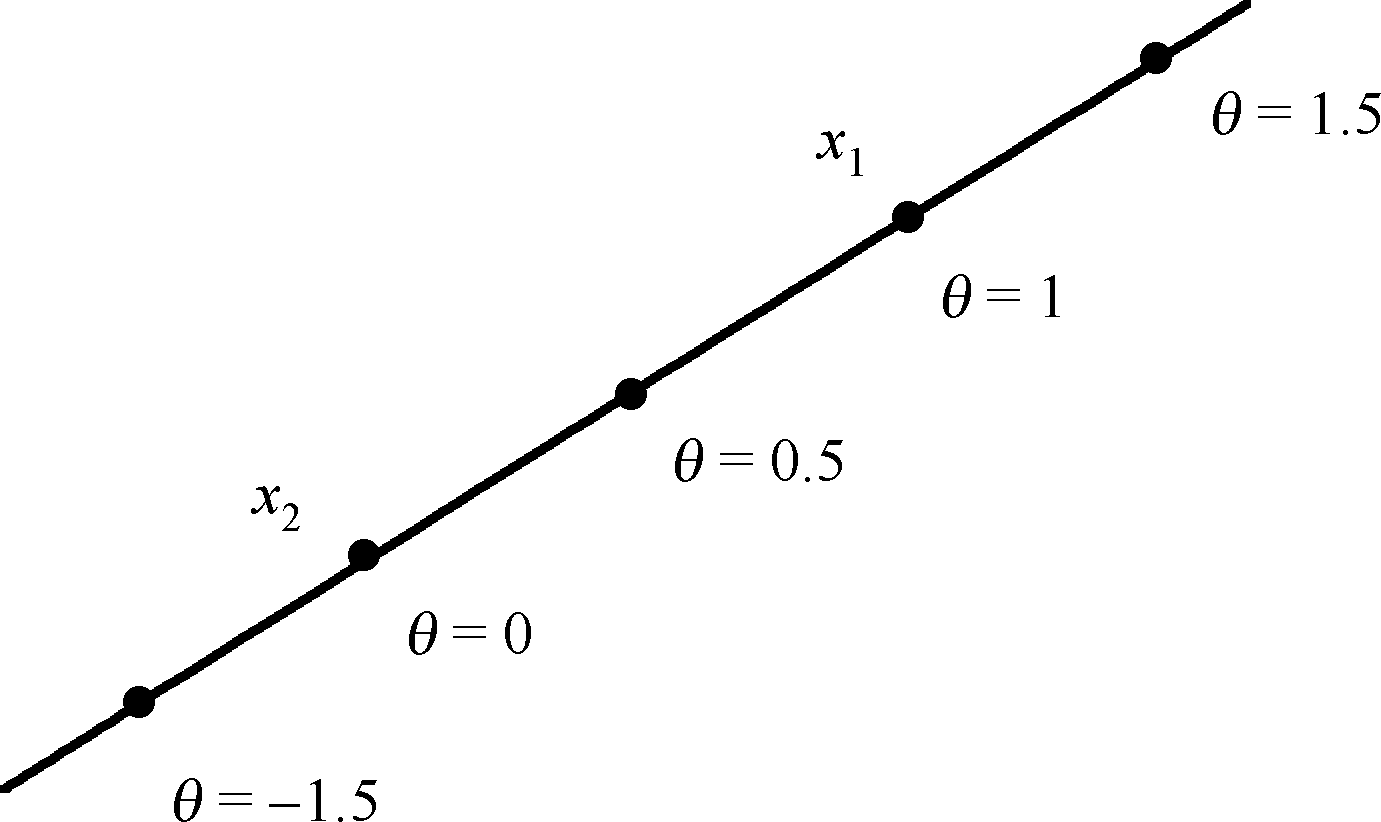
\includegraphics[height=4cm,width=6cm]{Ch2-affine-set.png}
%\caption{affine set}
\end{figure}
}


\onslide<2->{
\dred{仿射集}: 包含通过集合中任意两个不同点的线}
 

\onslide<3->{
\textbf{例如}: 线性方程的解集 $\{x \mid A x=b\}$

\hint{Q. 每个仿射集都可以表示为线性方程组的解集吗?}
}



\onslide<4->{
Q.	$x=\theta x_{1}+(1-\theta) x_{2}$ \quad \hint{($\theta \in [0,1]$)}, 
 {是什么样的集合?}
}
\end{frame}
%---------------------------------------------------------
\begin{frame}
\frametitle{凸集}

\begin{itemize}[<+->]
 \item \textbf{线段:} 在 $x_1$ 和 $x_2$之间: 所有点
\begin{equation}
x=\theta x_{1}+(1-\theta) x_{2}
\end{equation}
其中 $0 \leq \theta \leq 1$
\item
\textbf{凸集}: 包含集合中任意两点之间的线段
\begin{equation}
x_{1}, x_{2} \in C, \quad 0 \leq \theta \leq 1 \quad \Longrightarrow \quad \theta x_{1}+(1-\theta) x_{2} \in C
\end{equation}

\item
\textbf{例如:} (一个凸集, 两个非凸集)
\begin{figure}[htbp]
\centering
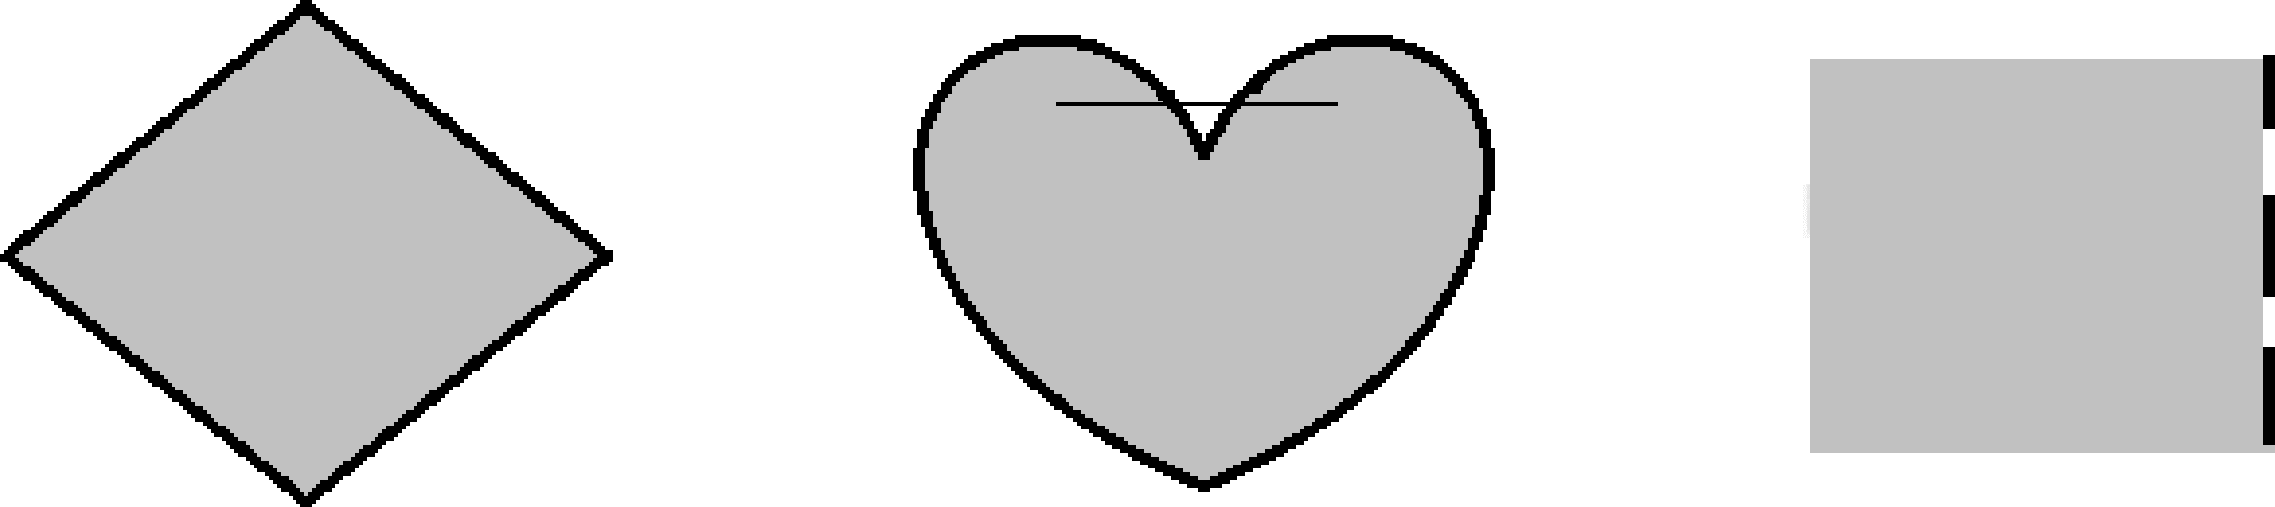
\includegraphics[width=8cm]{Ch2-Convex-set.png}
%\caption{affine set}
\end{figure}
\end{itemize}

\end{frame}
%-----------------------------------
\begin{frame}
\frametitle{凸组合和凸包}

\begin{itemize}
  \item \textbf{凸组合:}  $x_1,\cdots,x_k$的凸组合:  
\begin{equation}
x=\theta_{1} x_{1}+\theta_{2} x_{2}+\cdots+\theta_{k} x_{k}
\end{equation}
其中 $\theta_{1}+\cdots+\theta_{k}=1, \theta_{i} \geq 0$\\

 %\quad
\item
\textbf{凸包 conv} $S$:\\ $S$中所有凸组合的集合
\begin{figure}[htbp]
\centering
\includegraphics[width=7cm]{Ch2-Convex-hull.png}
%\caption{affine set}
\end{figure}

\end{itemize}
\end{frame}
%--------------------------------------------------
\begin{frame}
\frametitle{凸锥}

\begin{itemize}
  \item \textbf{$x_1$ 和 $x_2$的锥组合(非负线性组合)} : 对于点$x_1$ 和 $x_2$
\begin{equation}
x=\theta_{1} x_{1}+\theta_{2} x_{2}
\end{equation}
其中 $\theta_{1} \geq 0, \theta_{2} \geq 0$

\item E.g.
\begin{figure}[htbp]
\centering
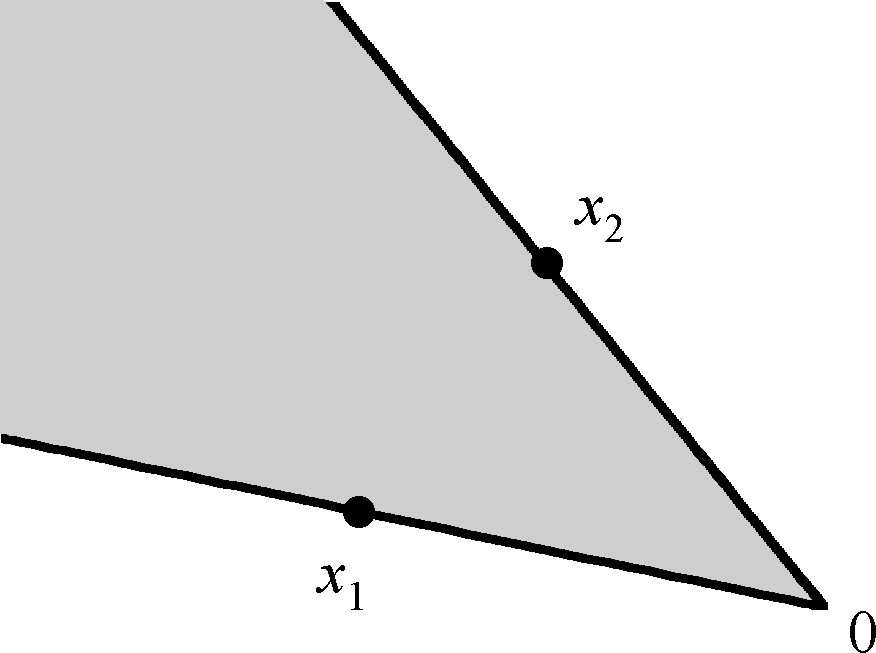
\includegraphics[width=0.3\textwidth]{Ch2-convex-cone.png}
%\caption{convex cone}
\end{figure}

\item
\textbf{凸锥}: 包含集合中所有元素的锥组合的集合
\end{itemize}

\end{frame}
%=================================================================
\subsection{一些重要的示例}
\begin{frame}
\frametitle{超平面和半空间}

\begin{itemize}%[<+->]
	\item<1-> 二维平面上的一条直面 将平面中分成两部分 
\item<2->
超平面: 具有以下形式的集合 $\left\{x \mid a^{T} x=b\right\}(a \neq 0)$


%\begin{figure}[htbp]
%\centering
%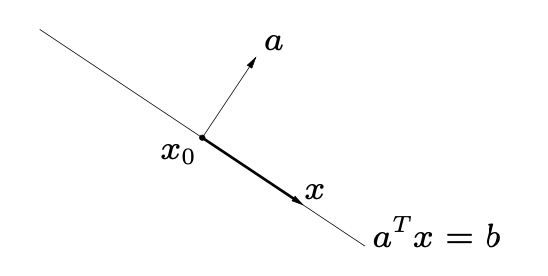
\includegraphics[height=3cm,width=4cm]{Ch2-Hyperplanes-1.png}
%\caption{Hyperplanes 1}
%\end{figure}

\item<2->
\textbf{半空间}: 具有以下形式的集合 $\left\{x \mid a^{T} x \leq b\right\} (a \neq 0)$,

%\item[] %\begin{figure}[htbp]
%\centering
%\includegraphics[height=3cm,width=4cm]{Ch2-Hyperplanes-2.png}
 %\caption{$a$ is the normal vector}
%\end{figure}


 \item<3-> 超平面是仿射集;半空间是凸的


\end{itemize}

\end{frame}
%---------------------------------------------------
\begin{frame}
\frametitle{欧氏球和椭球}

\begin{itemize}[<+->]
	\item 二维平面中的圆 和 椭圆 
  \item
\textbf{(欧几里德) 球:} 其中$x_c$ 是球心,$r$为半径:
\begin{equation}
B\left(x_{c}, r\right)=\left\{x \mid\left\|x-x_{c}\right\|_{2} \leq r\right\}=\left\{x_{c}+r u \mid\|u\|_{2} \leq 1\right\}
\end{equation}

\item \textbf{椭球:} 具有以下形式的集合
\begin{equation}
\left\{x \mid\left(x-x_{c}\right)^{T} P^{-1}\left(x-x_{c}\right) \leq 1\right\}
\end{equation}
其中 $P \in \mathbf{S}_{++}^{n}$($i.e.$, P为对称正定矩阵)

  \begin{figure}[htbp]
\centering
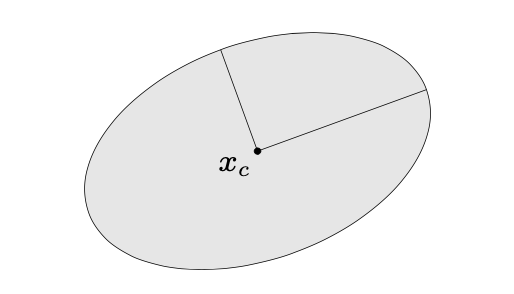
\includegraphics[width=3.5cm,angle=0.5]{Ch2-Euclidean.png}
%\caption{Euclidean balls and ellipsoids}
\end{figure}

\item 另一个表示: $\left\{x_{c}+A u \mid\|u\|_{2} \leq 1\right\}$,  $A$为正定矩阵


\end{itemize}
\end{frame}
%-----------------------------------------
\begin{frame}
	\frametitle{范数球和范数锥}

\begin{itemize}%[<+->]
  \item<1->
  \textbf{范数}:   $\|\cdot\|$ 满足:
	\begin{itemize}
		\item $\|x\| \geq 0 ;\|x\|=0$ 当且仅当 $x=0$
		\item $\|t x\|=|t|\|x\|$ 对于 $t \in \mathbb{R}$
		\item $\|x+y\| \leq\|x\|+\|y\|$
	\end{itemize}

%\item 符号: $\|\cdot\|$ 是一般(未指定)范数; $\|\cdot\|$ symb是特殊范数\\

\item<2-> \textbf{范数球}\ 球心 $x_{c}$ ,半径为 $r$ 的范数球:$\left\{x \mid\left\|x-x_{c}\right\| \leq r\right\}$

\item<3->
%\begin{columns}
%	\column{0.4\textwidth}
	\textbf{范数锥:} $\{(x, t) \mid\|x\| \leq t\}$
	
 \footnotehint{欧氏锥称为二阶锥}
 
%	\column{0.5\textwidth}
%	\begin{figure}[htbp]
%    \centering
%    \includegraphics[height=3cm,width=4cm]{Ch2-Norm-balls-and-norm-cones.png}
%    %\caption{Norm balls and norm cones}
%    \end{figure}
%\end{columns}

\hint{-范数球和范数锥是凸的}
\end{itemize}
\end{frame}
%-----------------------------------
\begin{frame}
	\frametitle{多面体}

\begin{itemize}[<+->]
  \item
	有限个线性不等式和等式的解集
\begin{equation}
	A x \preceq b, \quad C x=d
\end{equation}
$\left(A \in \mathbb{R}^{m \times n}, C \in\mathbb{R}^{p \times n}, \preceq\right.$ 是分量不等式)

\item[] \begin{figure}[htbp]
\centering
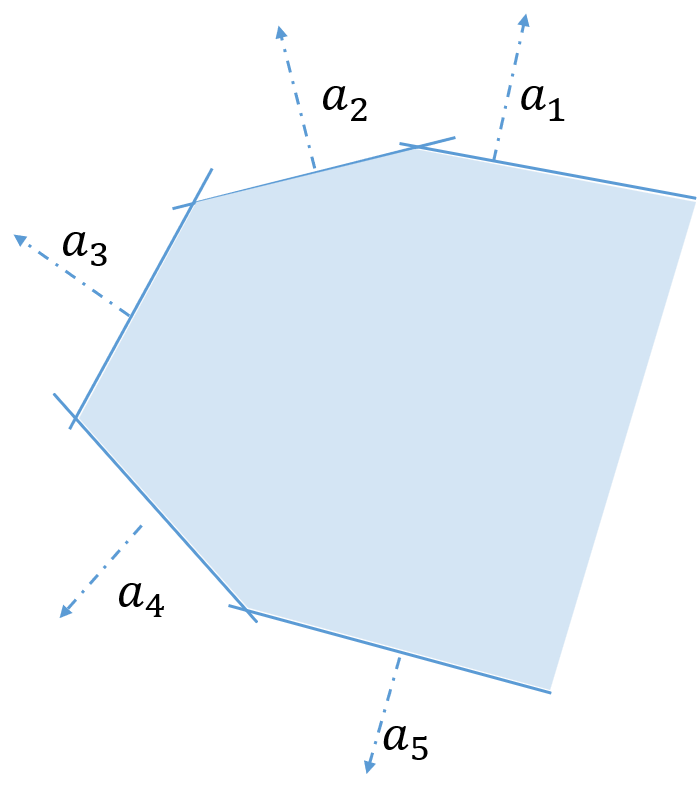
\includegraphics[height=4cm,width=5cm]{Ch2-Polyhedra.png}
%\caption{Polyhedra}
\end{figure}

\item
多面体是\hint{有限个}半空间和\hint{超平面}的\hint{交集}
\end{itemize}
\end{frame}
%--------------------------------
\begin{frame}
	\frametitle{正半定锥}
%	\textbf{符号:}
	\begin{itemize}[<+->]
		\item $\mathbf{S}^{n}$ 表示 $n \times n$ 对称矩阵的集合
		\item $\mathbf{S}_{+}^{n}=\left\{X \in \mathbf{S}^{n} \mid X \succeq 0\right\}:$ 表示 $n \times n$ 对称半正定矩阵的集合
		    \begin{equation}
			X \in \mathbf{S}_{+}^{n} \Longleftrightarrow z^{T} X z \geq 0  \quad { \forall }\, z
		    \end{equation}
	        $\mathbf{S}_{+}^{n}$ 是 凸锥
	    \item $\mathbf{S}_{++}^{n}=\left\{X \in \mathbf{S}^{n} \mid X \succ 0\right\}$: $n \times n$ 对称正定矩阵的集合

	
\item[]
%	\begin{columns}
%	\column{0.4\textwidth}
	\textbf{例如:} $\left[\begin{array}{ll}x & y \\ y & z\end{array}\right] \in \mathbf{S}_{+}^{2}$	
	
%	\bigskip
	
	\footnotehint{$x\geq0$, $xz-y^2\geq 0$}
%	\column{0.5\textwidth}
%	\begin{figure}[htbp]
%    \centering
%    \includegraphics[height=4cm,width=5cm]{Ch2-Positive-semidefinite-cone.png}
%    %\caption{Positive semidefinite cone}
%    \end{figure}
%\end{columns}
%\item \hint{Q. 图中的“内部点”是否包含在锥中?}
\end{itemize}
\end{frame}


\subsection{保持凸性的运算}
\begin{frame}
\frametitle{保持凸性的运算}

\dred{Q:如何检测一个集合 $C$是凸集合?如何构造凸集合? }

\begin{enumerate}[<+->]
\item 利用定义
\begin{equation}
	x_{1}, x_{2} \in C, \quad 0 \leq \theta \leq 1 \quad \Longrightarrow \quad \theta x_{1}+(1-\theta) x_{2} \in C
\end{equation}\\

\item \hint{证明 $C$是通过保持凸性的运算获得的:}  简单的凸集合(超平面、半空间、范数球等)$\rightarrow$复杂凸集合 
\bigskip
\begin{itemize}
	\item 交集
	\item 仿射变换
	\item 透视函数
	\item 线性分式映射
\end{itemize}
\end{enumerate}
\end{frame}
%-------------------------------------
\begin{frame}
\frametitle{交集}


\begin{itemize}[<+->]
  \item
\hint{定理:凸集合(任意数量)的交集是凸的。}


\item \tinyhint{证. 设$C_1,C_2$凸集合,$\forall x_1,x_2\in C_1\cap C_2 $,
	$\theta\in [0,1]$, 验证$\theta x_1 + (1-\theta)x_2 \in C_1\cap C_2$}
%\item
%\textbf{例如:}
%\begin{equation}
%	S=\left\{x \in \mathbb{R}^{m}|| p(t) \mid \leq 1 \text { for }|t| \leq \pi / 3\right\}
%\end{equation}
%其中 $p(t)=x_{1} \cos t+x_{2} \cos 2 t+\cdots+x_{m} \cos m t$\\
%
%\item $S = \cap_{|t|\leq \frac{\pi}{3}}^{} S_t$,\quad $S_t :=\{x | -1\leq (\cos t, \cdots, \cos mt)^{\top} x \leq 1 \}$.
%
%\item
%对于 $m=2$ :
%\begin{figure}[htbp]
%    \centering
%    \includegraphics[height=4cm,width=10cm]{Ch2-Intersection.png}
%    %\caption{Intersection}
%    \end{figure}


 \end{itemize}
\end{frame}
%------------------------------------------
\begin{frame}
	\frametitle{仿射变换}

\begin{itemize}
	\item \highlight{ 定义.} $\cala:\calx\rightarrow\caly$为仿射变换: $\forall x_1,x_2 
	\in \calx$, $\theta\in \bbr$, 
	有 $\cala(\theta x_1 + (1-\theta) x_2) = \theta  \cala x + (1-\theta) \cala x_2$
  \item
	如果 \hint{$f: \mathbb{R}^{n} \rightarrow \mathbb{R}^{m}$ 是仿射变换,} i.e.,
$ f(x)=A x+b $ , $ A \in \mathbb{R}^{m \times n}, b \in \mathbb{R}^{m} $
	\begin{enumerate}
		\item \hint{在$f$ 下的像集是凸集合}
		\begin{equation}
			S \subseteq \mathbb{R}^{n} \text { 凸 } \Longrightarrow f(S)=\{f(x) \mid x \in S\} \text { 凸 }
		\end{equation}
		\item \hint{ 在$f$下凸集的逆像$f^{-1}(C)$ 是凸的 ( proof. Ex.)}
		\begin{equation}
			C \subseteq \mathbb{R}^{m} \text {凸} \Longrightarrow f^{-1}(C)=\left\{x \in \mathbb{R}^{n} \mid f(x) \in C\right\} \text { 凸 }
		\end{equation}
	\end{enumerate}

\tinyhint{证. (1)  $\forall y_1,y_2\in f(S)$, 验证 $\theta y_1 + (1-\theta)y_2 \in f(S)$, $\theta\in(0,1)$}

\textbf{例}
\begin{itemize}
	\item 缩放、平移、投影
	\item 线性矩阵不等式的解集 $\left\{x \mid x_{1} A_{1}+\cdots+x_{m} A_{m} \preceq B\right\}$ ($\left.A_{i}, B \in \mathbf{S}^{p}\right)$
	\item 双曲线锥体 $\left\{x \mid x^{T} P x \leq\left(c^{T} x\right)^{2}, c^{T} x \geq 0\right\}$ ( $\left.P \in \mathbf{S}_{+}^{n}\right)$
\end{itemize}

\end{itemize}
\end{frame}


\begin{frame}

\begin{itemize}%[<+->]
  \item<only@1-2>
   \hint{缩放和平移}
   %If $S \subseteq \mathbf{R}^{n}$ is convex, $\alpha \in \mathbf{R}$, and $a \in \mathbf{R}^{n}$, then the sets $\alpha S$ and $S+a$ are convex, where
$$
\alpha S=\{\alpha x \mid x \in S\}, \quad S+a=\{x+a \mid x \in S\}
$$

\item<only@2-2>\hint{凸集在其某些坐标上的投影是凸的}: 若 $S \subseteq$ $\mathbf{R}^{m} \times \mathbf{R}^{n}$是凸的, 那么
$$
T=\left\{x_{1} \in \mathbf{R}^{m} \mid\left(x_{1}, x_{2}\right) \in S, x_{2} \in \mathbf{R}^{n}\right\}
$$
也是凸的.

\item<only@3-5> \hint{两个集合的和}
$$
S_{1}+S_{2}=\left\{x+y \mid x \in S_{1}, y \in S_{2}\right\}
$$

\item<only@3-3>[]  
\begin{figure}[H]
\begin{center}
  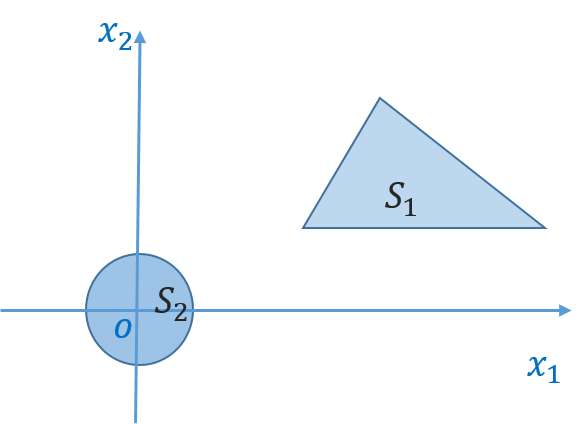
\includegraphics[width=0.4\textwidth]{S1-plus-S2}
\end{center}
\caption{思考 $S_1+S_2= ?$,  $S_2 =\epsilon \mathbf{B}$}
\end{figure}


%\item<only@4-5>
%如果 $S_{1}$ 和 $S_{2}$ 是凸的, 那么 $S_{1}+S_{2}$ 也是凸的.



\end{itemize}
\end{frame}

% ============== here ============
%-----------------------------------------
\begin{frame}
\frametitle{例.仿射变换与凸集}

\begin{itemize}
	 
\item 
如果 $S_{1}$ 和 $S_{2}$ 是凸的, 那么 $S_{1}+S_{2}$ 也是凸的.


 
\begin{footnotesize}证明. 如果 $S_{1}$ 和 $S_{2}$是凸的, 那么乘积或笛卡尔乘积也是凸的
$$
S_{1} \times S_{2}=\left\{\left(x_{1}, x_{2}\right) \mid x_{1} \in S_{1}, x_{2} \in S_{2}\right\}
$$
\footnotehint{该集合在线性函数下的图像 $f\left(x_{1}, x_{2}\right)=x_{1}+x_{2}$ 是总和 $S_{1}+S_{2}$. }
\end{footnotesize}

\item  \hint{部分和} $S_{1}, S_{2} \in \mathbf{R}^{n} \times \mathbf{R}^{m},$ 定义为
$$
S=\left\{\left(x, y_{1}+y_{2}\right) \mid\left(x, y_{1}\right) \in S_{1},\left(x, y_{2}\right) \in S_{2}\right\}
$$
其中 $x \in \mathbf{R}^{n}$ 且 $y_{i} \in \mathbf{R}^{m}$.

- 当 $m=0$, 部分和 $\rightarrow$交集 $S_{1}$ 和 $S_{2} ;$

- 当 $n=0,$ 部分和 $\rightarrow$集合加法.

- \footnotehint{两个凸集的部分和仍是凸集  }
\end{itemize}
\end{frame}

% ============== here ============
%-----------------------------------------
\begin{frame}
	\frametitle{透视函数(选讲)}

	\textbf{透视函数}$P: \mathbb{R}^{n+1} \rightarrow \mathbb{R}^{n}$
    \begin{equation}
	    P(x, t)=x / t, \quad  P=\{(x, t) \mid t>0\}
    \end{equation}
 
透视下凸集的图像和逆像是凸集.

\onslide<2->{
%\begin{figure}[htb]
\begin{center}
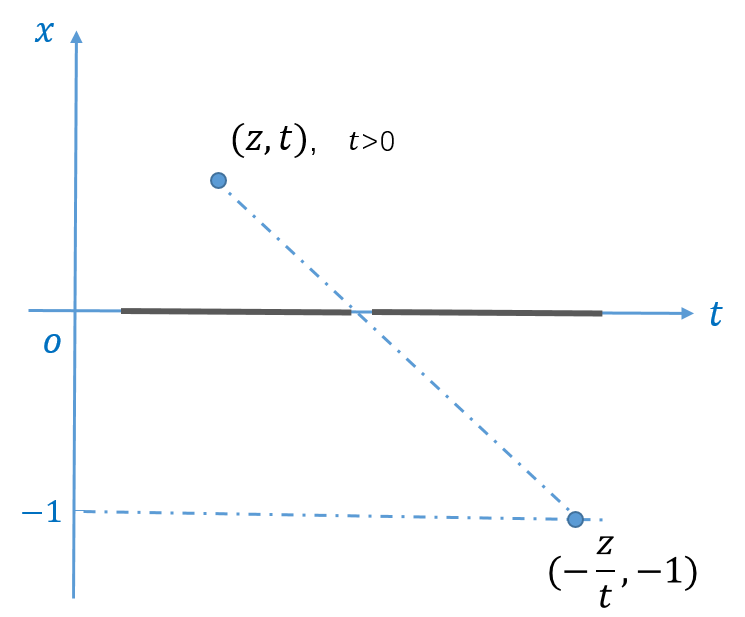
\includegraphics[width = 0.4\textwidth]{figure/ch2-perspective-fun}

\hint{透视函数:针孔照相机的动作 }
\end{center}

%\caption{Perspective function: the action of a pin-hole camera. }
%\end{figure}
}

\end{frame}


\begin{frame}
	\frametitle{透视函数和线性分式映射}


\textbf{线性分式映射} $f: \mathbb{R}^{n} \rightarrow \mathbb{R}^{m}:$
\begin{equation}
	f(x)=\frac{A x+b}{c^{T} x+d}, \quad \ \ f=\left\{x \mid c^{T} x+d>0\right\}
\end{equation}

\hint{命题}
线性分式映射下凸集的图像和逆像是凸集。

%\end{itemize}
\end{frame}
%------------------------
%\begin{frame}
%	\frametitle{透视函数和线性分段函数}
%	\textbf{线性分段函数的例子}
%    \begin{equation}
%	    f(x)=\frac{1}{x_{1}+x_{2}+1} x
%    \end{equation}\\
%    \bigskip
%    \begin{figure}[htbp]
%    \centering
%    \includegraphics[height=6cm,width=10cm]{Ch2-Perspective-and-linear-fractional-function.png}
%    %\caption{Perspective and linear-fractional function}
%    \end{figure}
%\end{frame}
%====================================================================

\subsection{广义不等式}

\begin{frame}
\frametitle{广义不等式:动机}

Q. 比较两个大小 $a$ 和 $b$? 
\begin{itemize}
  \item 两个数字 $a$, $b$ 
  
     $2<3 $ 
  
  \item  $a,b\in \bbr^2$ 
  
    $(1,2)\prec (3,4)$ 
  
  \item $A,B \in \mathbf{S}_{}^{n}$ ? 
  
\end{itemize}


\end{frame}

\begin{frame}
\frametitle{广义不等式:动机}

Q. 比较   $a$ 和 $b$?
\begin{itemize}
  \item 两个真实数字 $a$, $b$

     $2<3 $ $\Leftrightarrow$ $3-2 \in \textbf{整数} K$, $K = [0,\infty)$

  \item  $a,b\in \bbr^2$

    $(1,2)\prec (3,4)$ $\Leftrightarrow$ $(3,4)-(1,2) \in \textbf{整数} K$, $K = \mathbb{R}_{+}^2$

  \item $A,B \in \mathbf{S}_{}^{n}$ ?
  
   $A\prec B $ $\Leftrightarrow$ $B-A \in \textbf{整数} K$, $K = \mathbf{S}_{+}^n$

\end{itemize}


\end{frame}

\begin{frame}
\frametitle{广义不等式}

\hint{定义. }
凸锥 $K \subseteq \mathbb{R}^{n}$ 称为 \textbf{正常锥(proper cone)}, 若 
\begin{itemize}
	\item $K$ 是封闭的 (有边界)
	\item $K$是实心的 (内部不是空的)
	\item $K$ 不包含直线 
\end{itemize}



\onslide<2->{\textbf{实例}}
\begin{itemize}
	\item<2-> 非负整数 $K=\mathbb{R}_{+}^{n}=\left\{x \in \mathbb{R}^{n} \mid x_{i} \geq 0, i=1, \ldots, n\right\}$
	\item<3-> 半正定锥 $K=\mathbf{S}_{+}^{n}$
	\item<4->  
	$[0,1]$上的非负多项式:
	\begin{equation}
		K=\left\{x \in \mathbb{R}^{n} \mid x_{1}+x_{2} t+x_{3} t^{2}+\cdots+x_{n} t^{n-1} \geq 0,  t \in[0,1]\right\}
	\end{equation}
\end{itemize}
\end{frame}
%-----------------------------
\begin{frame}
	\frametitle{广义不等式}
	\textbf{广义不等式} 由正常锥$K$定义 :
\begin{equation}
	x \preceq_{K} y \quad \Longleftrightarrow \quad y-x \in K, \quad \quad x \prec_{K} y \quad \Longleftrightarrow \quad y-x \in \textbf { 整数 } K
\end{equation}\\
\bigskip
\textbf{实例}
\begin{itemize}
	\item<2-> 分量不等式 $\left(K=\mathbb{R}_{+}^{n}\right)$
    \begin{equation}
    	x \preceq_{\mathbb{R}_{+}^{n}} y \quad \Longleftrightarrow \quad x_{i} \leq y_{i}, \quad i=1, \ldots, n
    \end{equation}
    \item<3-> 矩阵不等式 $\left(K=\mathbf{S}_{+}^{n}\right)$
    \begin{equation}
    	X \preceq_{\mathbf{s}_{+}^{n}} Y \Longleftrightarrow Y-X \text { 半正定 }
    \end{equation}
    %这两种类型非常常见,因此我们删除了 $\preceq_{K}$中的下标
\end{itemize}
\bigskip
\onslide<4->{
\textbf{特性:}  $\preceq_{K}$ 
  的很多特性与 $\leq$ 在 $\mathbb{R}$上的性质相似,  $e.g.$,
\begin{equation}
	x \preceq_{K} y, \quad u \preceq_{K} v \quad \Longrightarrow \quad x+u \preceq_{K} y+v
\end{equation}
}
\end{frame}
%-----------------------------------
%\begin{frame}
%	\frametitle{最小元和极小元}
%	$\preceq_{K}$ 通常不是全序: 可能出现 $x \npreceq_{K} y$ 且 $y \npreceq_{K} x$\\
%	\bigskip
%\onslide<2->{
%    $x \in S$ 是$S$ 关于 $\preceq_{K}$的一个 \textbf{minimum element (最小点)} ,  如果
%    \begin{equation}
%    \forall\ 	y \in S \quad \Longrightarrow \quad x \preceq_{K} y
%    \end{equation}\\
%}
% \onslide<3->{   \bigskip
%    $x \in S$ 是 $S$关于 $\preceq_{K}$ 的一个 \textbf{minimal element (极小点)},如果
%    \begin{equation}
%    \forall\ 	y \in S, \quad y \preceq_K x \quad \Longrightarrow \quad y=x
%    \end{equation}
%    }
%    \begin{columns}
%	\column{0.45\textwidth}
%\onslide<4->{
%	\textbf{例子:}
%	 $\left(K=R_{+}^{2}\right)$\\
% }
%      \onslide<5->{  $x_{1}$ 是 $S_{1}$的最小点 \\$x_{2}$ 是$S_{2}$的极小点
%     }
%	\column{0.45\textwidth}
%\onslide<4->{
%	\begin{figure}[htbp]
%    \centering
%    \includegraphics[height=4cm,width=6cm]{Ch2-Minimum-and-minimal-elements.png}
%    %\caption{Minimum and minimal elements}
%    \end{figure}
%    }
%\end{columns}
%\end{frame}
%====================================================================


\subsection{分离和支撑超平面}
\begin{frame}
\frametitle{超平面分割定理}

\hint{定理. [超平面分割定理]}
如果$C$和$D$是非空不相交凸集,则存在$a \neq 0, b$: 
\bigskip
\begin{equation}\label{eq-seperation}
	a^{T} x \leq b  \forall   x \in C, \quad a^{T} x \geq b \forall x \in D
\end{equation}
\begin{figure}[htbp]
    \centering
    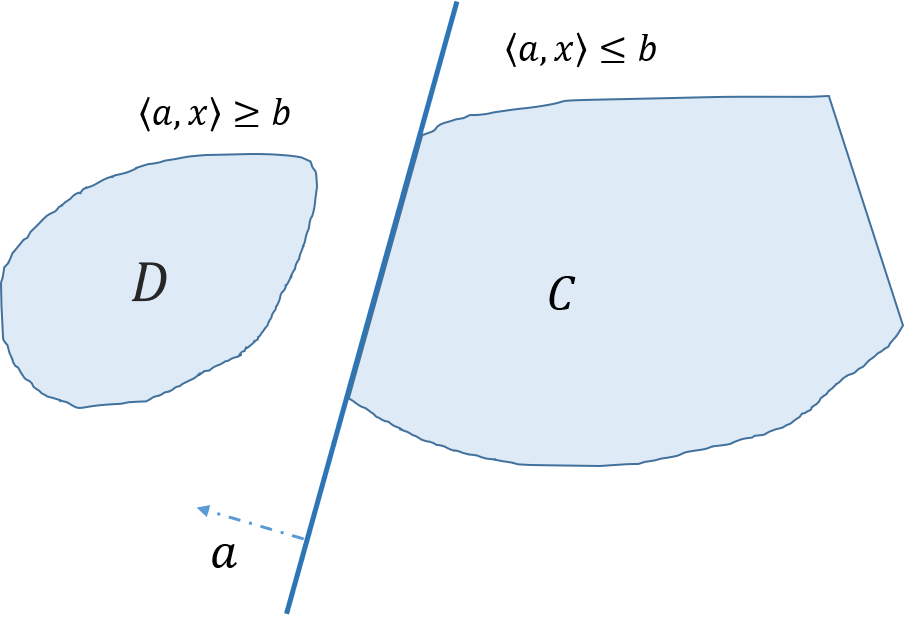
\includegraphics[height=4cm,width=7cm]{Ch2-Separating-hyperplane-theorem.png}
    %\caption{Separating hyperplane theorem}
    \end{figure}

\hint{定义}  若(\ref{eq-seperation})成立,称超平面 $\left\{x \mid a^{T} x=b\right\}$分离 $C$ 和 $D$


\onslide<2->{ 
\hint{定义. 严格的分离} 若存在$a \neq 0, b$:	$a^{T} x < b , \forall   x \in C, \quad a^{T} x > b \forall x \in D$,称超平面 $\left\{x \mid a^{T} x=b\right\}$严格的分离集合 $C$ 和 $D$

%需要额外的假设 (例如, $C$ 是封闭的, $D$ 是单例的(singleton))
}

\end{frame}
%-----------------------------------


\begin{frame}
  \hint{例子} [点和闭凸集的严格分离]
  假设$C$是一个闭凸集,
  $x_0 \not\in C$

  $\Rightarrow$ $x_0$ 和 $C$ 可以严格分开.


  \bigskip
\onslide<2->{
 \hint{推论}
   闭凸集是包含它的所有半空间的交集。
 }

\end{frame}


\begin{frame}
	\frametitle{支撑超平面定理}
	\hint{定义.}  $C$在边界点$x_{0}$处 的\textbf{支撑超平面}:
\begin{equation}
	\left\{x \mid a^{T} x=a^{T} x_{0}\right\}
\end{equation}
对于所有的 $x \in C$ 当 $a \neq 0$ 并且 $a^{T} x \leq a^{T} x_{0}$ 

\onslide<2->{
 \bigskip
 \hint{定理}  [支撑超平面定理] 如果$C$ 是凸的 $\Rightarrow$   $C$的每个边界点上存在一个支撑超平面.
 }

 \begin{figure}[htbp]
    \centering
    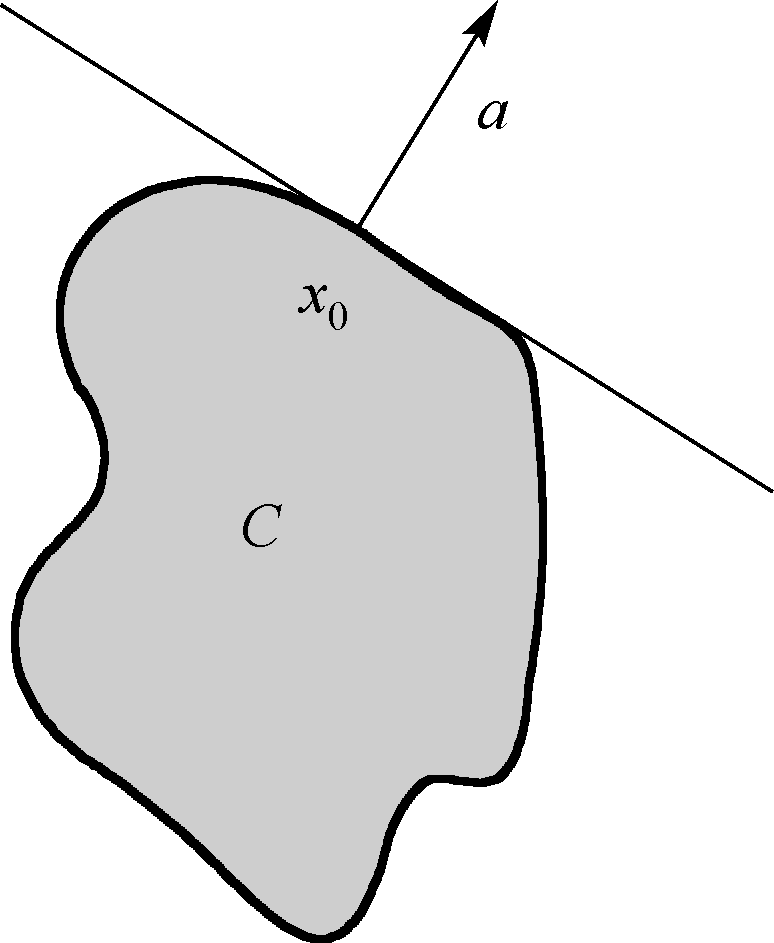
\includegraphics[height=4cm]{Ch2-Supporting-hyperplane-theorem.png}
    %\caption{Separating hyperplane theorem}
    \end{figure}
\end{frame}

\begin{frame}
	\frametitle{支撑超平面 }

 取 $f: \mathbb{R}\rightarrow \mathbb{R}$, $f(x) = |x|$. 考虑其支撑超平面(线) $\textnormal{epi} f = \{(x,t)\in \bbr^2| t\geq |x|\}$ at $(0,0)$.

\begin{itemize}[<+->]
  \item 直线的斜率是多少?
  \item 切线蕴含导数 $\rightarrow$ 支撑超平面 蕴含凸函数的(次)微分. 
  
   $$
   \partial f(0) = [-1,1]. 
   $$
\end{itemize}

\end{frame}


%====================================================================
\subsection{对偶锥与广义不等式}
\begin{frame}
\frametitle{对偶锥与广义不等式}

\begin{itemize}[<+-> ]
\item\hint{定义.}
$K$ 的\textbf{对偶锥} :
\begin{equation}
	K^{*}=\left\{y \mid y^{T} x \geq 0 \text { for all } x \in K\right\}
\end{equation}\\
%\bigskip
\item  \hint{示例}
\begin{itemize}
	\item 负值集合. $ K=\mathbb{R}_{+}^{n}: K^{*}=\mathbb{R}_{+}^{n}$
    \item 半正定锥.
     $ K=\mathbf{S}_{+}^{n}: K^{*}=\mathbf{S}_{+}^{n}$
    \item 标准圆锥面 $K=\left\{(x, t) \mid\|x\|_{2} \leq t\right\}: K^{*}=\left\{(x, t) \mid\|x\|_{2} \leq t\right\}$
    \item 标准圆锥面 $K=\left\{(x, t) \mid\|x\|_{1} \leq t\right\}: K^{*}=\left\{(x, t) \mid\|x\|_{\infty} \leq t\right\}$
\item 前三个例子是锥 \textbf{自对偶} 锥
\end{itemize}

\item 正常锥的对偶锥是正常锥,因此定义了广义不等式
   \begin{equation}
	y \succeq_{K^{*}} 0 \quad \Longleftrightarrow \quad y^{T} x \geq 0 \text { 对于所有 } x \succeq_{K} 0
    \end{equation}
\end{itemize}

\end{frame}
%%------------------------------------------
%\begin{frame}
%	\frametitle{Minimum and minimal elements via dual inequalities}
%	\begin{columns}
%	\column{0.4\textwidth}
%	\textbf{minimum element} w.r.t. $\preceq K$\\
%    $x$ is minimum element of $S$ iff for all
%    $\lambda \succ_{K^{*}} 0, x$ is the unique minimizer of $\lambda^{T} z$ over $S$
%	\column{0.5\textwidth}
%	\begin{figure}[htbp]
%    \centering
%    \includegraphics[height=4cm,width=6cm]{Ch2-Minimum-and-minimal-elements-via-dual-inequalities.png}
%    %\caption{Minimum and minimal elements}
%    \end{figure}
%    \end{columns}
%    \textbf{minimal element} w.r.t. $\preceq K$
%    \begin{itemize}
%    	\item if $x$ minimizes $\lambda^{T} z$ over $S$ for some $\lambda \succ_{K^{*}} 0$, then $x$ is minimal
%    	\begin{figure}[htbp]
%        \centering
%        \includegraphics[height=3cm,width=6cm]{Ch2-Minimum-and-minimal-elements-via-dual-inequalities-2.png}
%        %\caption{Minimum and minimal elements 2}
%        \end{figure}
%    	\item if $x$ is a minimal element of a convex set $S,$ then there exists a nonzero $\lambda \succeq_{K^{*}} 0$ such that $x$ minimizes $\lambda^{T} z$ over $S$
%    \end{itemize}
%\end{frame}
%-----------------------------------------
%\begin{frame}
%	\frametitle{Minimum and minimal elements via dual inequalities}
%	\textbf{optimal production frontier}
%	\begin{itemize}
%		\item different production methods use different amounts of resources $x \in \mathbb{R}^{n}$
%		\item production set $P:$ resource vectors $x$ for all possible production methods
%		\item efficient (Pareto optimal) methods correspond to resource vectors $x$ that are minimal w.r.t. $\mathbb{R}_{+}^{n}$
%	\end{itemize}
%	\bigskip
%	\begin{columns}
%	\column{0.4\textwidth}
%	\textbf{example}$(n=2)$\\
%    $x_1, x_2, x_3$ are efficient; $x_4, x_5$ are not
%	\column{0.5\textwidth}
%	\begin{figure}[htbp]
%    \centering
%    \includegraphics[height=5cm,width=6cm]{Ch2-Minimum-and-minimal-elements-via-dual-inequalities-3.png}
%    %\caption{Minimum and minimal elements 3}
%    \end{figure}
%    \end{columns}
%\end{frame}

\begin{frame}
  \frametitle{总结:凸集 }

  \begin{itemize}
    \item<only@2>  \hint{定义.} 仿射集与凸集
    \item<only@2> \hint{例子.}
   超平面、半空间、球、椭球和椭圆、多面体

      \hint{凸锥: }  $\mathbf{R}_{+}^n$, $\mathbf{S}_{+}^n$, 范数锥



\item<only@2> 保持凸性的操作
     \begin{itemize}
       \item 交:       例\doublestar 多面体,半正定矩阵 $\bfS_{+}^{n}$

       \item 仿射变换的图像(和逆图像)

          例,\doublestar $\alpha S$, $S+a$, $S_1 + S_2$

          例, 部分和,线性矩阵不等式的解集,椭球

       \item 透视映射: $P(x,t) = x/t$, $t>0$,
      透视映射的图像(和逆图像)

       \item 线性分数映射: 
         $ f(x) = \frac{Ax+b}{c^Tx+d}$, $c^Tx+d >0$.



     \end{itemize}

     \item<only@3> 广义不等式
     \begin{itemize}
       \item \hint{正常锥:} 闭的,实心的, 不含直线
         \smallhint{例, $\bfR_{+}^n$, $\bfS^n_{+}$}

   \item 广义不等式:  
        $x\preceq_{K}^{} y \Leftrightarrow y-x \in K$, \quad 
        $x\prec_{K}^{} y \Leftrightarrow y-x\in\mathnormal{int}\,K$

      \item 最小元和极小元

     \end{itemize}
 
\end{itemize}
\end{frame}

\begin{frame}
	\frametitle{总结:凸集 }

\begin{itemize}
\item 超平面分割定理

\begin{itemize}
  \item 定义.\mystar(严格)分离的凸集 $C$ 和 $D$

  \item 定义.\mystar $x_0 \in \mathbf{bd}\,C$处的支撑超平面 $C$: $$\{x|\langle a,x\rangle = a^T x_0\}, $$ 其中
      $\langle a,x\rangle \leq  a^T x_0, \forall x\in C
      $

\item 例如, 闭凸集和外面与其不相交的一个点可以严格分离。

  推论:    闭凸集是包含它的所有半空间的交集。

\item 定理. 凸集$C$ $\Rightarrow$   $C$的每个边界点上均存在一个支撑超平面



\end{itemize}

\item  对偶锥与广义不等式

\begin{itemize}
  \item 对偶锥 $K$:\mystar $K^* = \{ y | \langle y,x\rangle \geq 0, \forall x \in K\}$.

\item 例, $\left(\bbr^n_+\right)^* = \bbr^n_{+}$, $\left(\bfS^n_+\right)^* = \bfS^n_{+}$


\item 例,               $\rightarrow$  范数  $\|\cdot\|_1 $ 对应的范数锥的对偶锥:  $\|\cdot\|_{\infty}$ 对应的锥 \mystar
\end{itemize}


  \end{itemize}
\end{frame}


\begin{frame}[allowframebreaks]
  \frametitle{练习题 }

  \begin{enumerate}
    \item  证明:所有$n$阶半正定矩阵的全体构成凸锥.

    \item 证明一个集合是凸集当且仅当它与任意直线的交是凸的。证明一个集合是仿射 的, 当且仅当它与任意直线的交是仿射的。

    \item 两个平行的超平面 $\left\{\mathbf{x} \in \mathbf{R}^{n} \mid \mathbf{a}^{\mathrm{T}} \mathbf{x}=b_{1}\right\}$ 和 $\left\{\mathbf{x} \in \mathbf{R}^{n} \mid \mathbf{a}^{\mathrm{T}} \mathbf{x}=b_{2}\right\}$ 之间的距离是多 少?

       \item  半空间的Voronoi描述。令 $\mathbf{a}$ 和 $\mathbf{b}$ 为 $\mathbf{R}^{\mathrm{n}}$ 上互异的两点。证明所有距离 $\mathbf{a}$ 比距离 $\mathbf{b}$ 近(Euclid 范数下)的点的集合,即 $\left\{\mathbf{x}\|\mathbf{x}-\mathbf{a}\|_{2} \leq\|\mathbf{x}-\mathbf{b}\|_{2}\right\}$, 是一个超平面。 用形如 $\mathbf{c}^{\mathrm{T}} \mathbf{x} \leq d$ 的不等式进行显式表示并绘出图像。

   \item   设 $\mathbf{C} \subseteq \mathbf{R}^{\mathbf{n}}$ 为一个凸集且 $x_{1}, \cdots, x_{k} \in \mathbf{C} .$
     令 $\theta_{1}, \cdots, \theta_{k} \in \boldsymbol{R}$ 满足 $\theta_{i} \geq 0, \theta_{1}+\cdots+\theta_{k}=1$.

  证明 $\theta_{1} x_{1}+\cdots+\theta_{k} x_{k} \in \mathbf{C}$. (凸性的定义是指此式在 $k=2$ 时成立; 你需要证明 对任意 $k$ 的情况。提示:对 $k$ 进行归纳。)

  \item  证明如果 $\mathbf{S}_{\mathbf{1}}$ 和 $\mathbf{S}_{2}$ 是 $\mathbf{R}^{\mathbf{m} \times \mathrm{n}}$ 中的凸集, 那么它们的部分和
$$
\mathbf{S}=\left\{\left(\mathbf{x}, \mathbf{y}_{\mathbf{1}}+\mathbf{y}_{2}\right) \mid \mathbf{x} \in \mathbf{R}^{\mathbf{m}}, \mathbf{y}_{1}, \mathbf{y}_{\mathbf{2}} \in \mathbf{R}^{\mathbf{n}}, \quad\left(\mathbf{x}, \mathbf{y}_{1}\right) \in \mathbf{S}_{\mathbf{1}},\left(\mathbf{x}, \mathbf{y}_{2}\right) \in \mathbf{S}_{\mathbf{2}}\right\}
$$
也是凸的。



 \item   支撑超平面。
(a)将闭凸集 $\left\{\mathbf{x} \in \mathbf{R}_{+}^{2}\right.$ | $\left.x_{1} x_{2} \geq 1\right\}$ 表示为半空间的交集。
(b)令 $\mathbf{C}=\left\{\mathbf{x} \in \mathbf{R}^{\mathbf{n}} \mid\|\mathbf{x}\|_{\infty} \leq 1\right\}$ 表示 $\mathbf{R}^{\mathrm{n}}$ 空间中的单位 $\ell_{\infty}-$ 范数球, 并令 $\hat{\mathbf{x}}$ 为 $\mathbf{C}$ 的边 界上的点。显式地写出集合 $\mathbf{C}$ 在 $\hat{\mathbf{x}}$ 处的支撑超平面。
 \item  支撑超平面定理的逆定理。
设集合 $\mathbf{C}$ 是闭的、含有非空内部并且在其边界上的每一点都有支撑超平面。证明 C 是凸集。
 \item   给出两个不相交的闭凸集不能被严格分离的例子。
 \item  支撑函数。集合 $\mathbf{C} \subseteq \mathbf{R}^{\mathbf{n}}$ 的支撑函数定义为
$$
\mathbf{S}_{\mathbf{C}}(\mathbf{y})=\sup \left\{\mathbf{y}^{\mathbf{T}} \mathbf{x} \mid \mathbf{x} \in \mathbf{C}\right\}
$$
(我们允许 $\mathbf{S}_{\mathbf{C}}(\mathbf{y})$ 取值为 $+\infty$.)设 $\mathbf{C}$ 和 $\mathbf{D}$ 是 $\mathbf{R}^{\mathrm{n}}$ 上的闭凸集。证明 $\mathbf{C}=\mathbf{D}$ 当且仅当 它们的支撑函数相等。

   \item 计算  $\{\mathrm{Ax} \mid \mathbf{x}>0\} \text { 的对偶雉, 其中 } \mathrm{A} \in \mathbf{R}^{\mathrm{mxn}} \text {. }$
  \end{enumerate}

\end{frame}



%\end{CJK*}
\end{document}
